\documentclass{article}
\usepackage[utf8]{inputenc}

% Page setup
\usepackage[a4paper,landscape,margin=2cm]{geometry}
\usepackage{amsmath}

% Typography
\usepackage[scaled]{helvet}
\let\familydefault\sfdefault

\usepackage[usenames,svgnames]{xcolor}
\usepackage{tikz,pgfplots}
\usetikzlibrary{positioning,arrows,intersections,calc}

\definecolor{colorwhite}     {RGB}{255,255,255}
\definecolor{colorserver}    {RGB}{199,212,104}
\definecolor{colorinterface} {RGB}{ 79,142,209}
\definecolor{colorcost}       {RGB}{143,232,186}
\definecolor{colortext}      {RGB}{ 29, 29, 27}
\definecolor{colorkey}       {RGB}{129, 29, 27}
\definecolor{colorclient}    {RGB}{190, 22, 34}

\begin{document}
\pagestyle{empty}
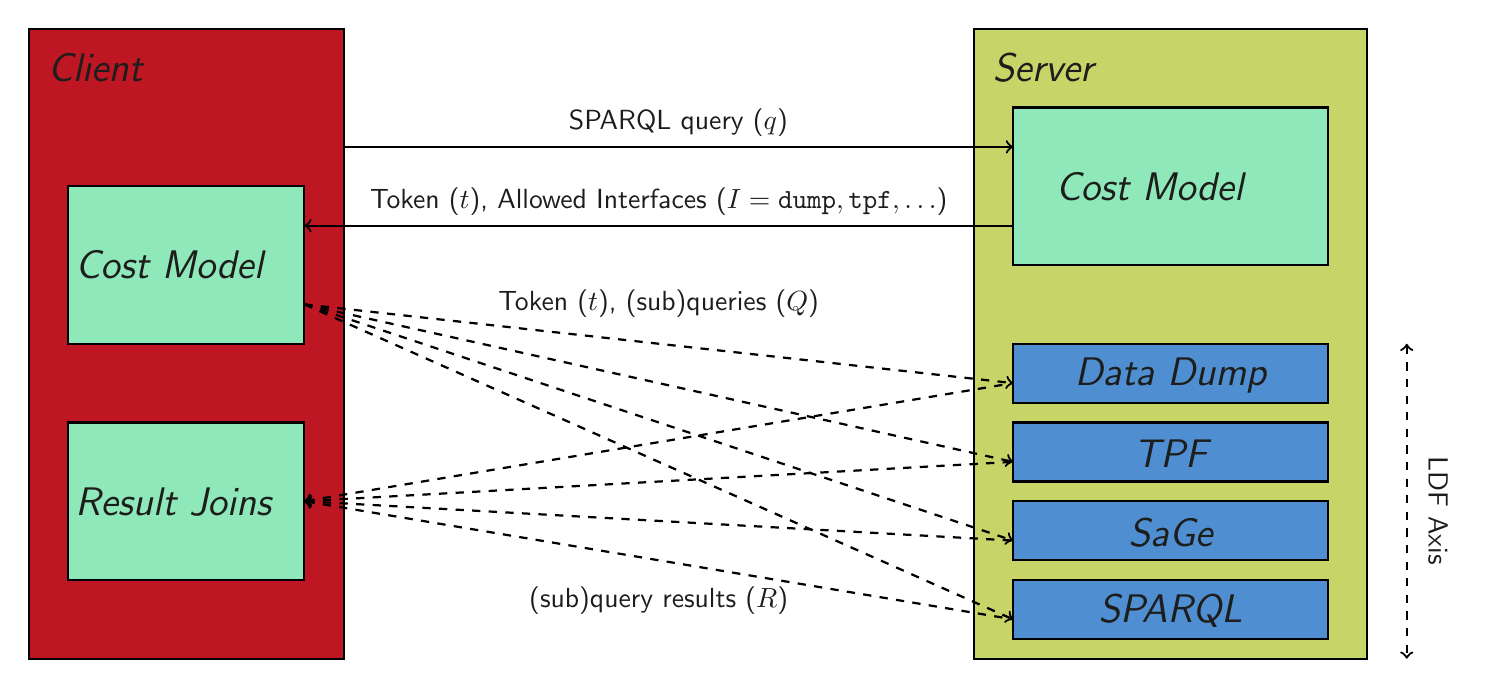
\begin{tikzpicture}[
    node distance = 10em, auto, thick,
    title/.style={text=colortext,font={\Large\itshape}},
    person/.style={text=colorwhite,font={\Large\bfseries}},
    code/.style={text=colortext,font={}},
    key/.style={text=colorkey,font={\tiny\itshape}}
]
    % Client
    \draw[fill=colorclient] (2,2) rectangle (-2,-6);
    \node[title,text width=10em] at (0,1.5) {Client};

    % Server
    \draw[fill=colorserver] (10,2) rectangle (15,-6);
    \node[title,text width=10em] at (12,1.5) {Server};
    
    % Server cost model
    \draw[fill=colorcost] (10.5,1) rectangle (14.5,-1);
    \node[title,text width=10em] at (12.8,0) {Cost Model};

    % Arrows between cost models
    \draw[->,thick](2,0.5) to node[midway,code] {SPARQL query ($q$)} (10.5,0.5);
    \draw[<-,thick](1.5,-0.5) to node[midway,code] {Token ($t$), Allowed Interfaces ($I = \texttt{dump}, \texttt{tpf}, \ldots$)} (10.5,-0.5);
    
    % Client cost model
    \draw[fill=colorcost] (-1.5,0) rectangle (1.5,-2);
    \node[title,text width=10em] at (0.35,-1) {Cost Model};
    
    % Interfaces
    \draw[fill=colorinterface] (10.5,-2) rectangle (14.5,-2.75);
    \node[title] at (12.5,-2.4) {Data Dump};
    \draw[fill=colorinterface] (10.5,-3) rectangle (14.5,-3.75);
    \node[title] at (12.5,-3.4) {TPF};
    \draw[fill=colorinterface] (10.5,-4) rectangle (14.5,-4.75);
    \node[title] at (12.5,-4.4) {SaGe};
    \draw[fill=colorinterface] (10.5,-5) rectangle (14.5,-5.75);
    \node[title] at (12.5,-5.4) {SPARQL};
    
    % Arrows to interfaces
    \draw[->,thick,dashed](1.5,-1.5) to node[above,code,yshift=0.2cm] {Token ($t$), (sub)queries ($Q$)} (10.5,-2.5);
    \draw[->,thick,dashed](1.5,-1.5) to (10.5,-3.5);
    \draw[->,thick,dashed](1.5,-1.5) to (10.5,-4.5);
    \draw[->,thick,dashed](1.5,-1.5) to (10.5,-5.5);
    
    % Client post processing
    \draw[fill=colorcost] (-1.5,-3) rectangle (1.5,-5);
    \node[title,text width=10em] at (0.35,-4) {Result Joins};
    
    % Arrows to client
    \draw[<-,thick,dashed](1.5,-4) to (10.5,-2.5);
    \draw[<-,thick,dashed](1.5,-4) to (10.5,-3.5);
    \draw[<-,thick,dashed](1.5,-4) to (10.5,-4.5);
    \draw[<-,thick,dashed](1.5,-4) to node[below,code,yshift=-0.2cm] {(sub)query results ($R$)} (10.5,-5.5);
    
    % LDF Axis
    \draw[<->,thick,dashed](15.5,-2) to node[code,yshift=0.7cm,xshift=0.4cm,rotate=-90] {LDF Axis} (15.5,-6);

\end{tikzpicture}
\end{document}
